\documentclass[xcolor=table]{beamer}


\let\Tiny=\tiny

\usepackage[russian]{babel}
\usepackage{cmap}
\usepackage[utf8]{inputenc}
\usepackage{amsmath}
\usepackage{color}
\usepackage[table]{xcolor}
%\usepackage{subfig}
\title[]{Интеллектуальный анализ данных\\(Data mining)}

% Don`t know how to make title slide properly using beamer customization :(
\author[]{ \\[0.5cm]  \Large Доклад на семинаре по \\ специальности \\[1.3cm]  Студент гр.4057/2 Виктор Смолов \\ 21 декабря 2010}

\usetheme{Darmstadt}
\usecolortheme{crane}
\useoutertheme{infolines} 
\setbeamersize{text margin left=1cm,text margin right=.5cm} 
\setbeamertemplate{navigation symbols}{}
\setbeamertemplate{headline}{}
\setbeamertemplate{footline}[page number]{}
\setbeamertemplate{caption}[numbered]

\newtheorem{defn}{Определение}
\newtheorem{prob}{Постановка задачи}

\definecolor{myGreen}{RGB}{0,201,94}
\definecolor{cell1}{RGB}{206,161,255}
\definecolor{cell2}{RGB}{160,222,176}

%{%
%\begin{flushright}{\begin{tt}\begin{LARGE}\insertframenumber/\inserttotalframenumber\end{LARGE}\end{tt}}\end{flushright}%
%}

\date[21 декабря 2010]{}
\begin{document}

\thispagestyle{empty}

\begin{frame}
  \maketitle
\end{frame}

\setcounter{page}{1}

\begin{frame}
  \frametitle{Содержание} 
  Введение \\[0.15cm]
  \tableofcontents
  Заключение \\[0.15cm]
  Список литературы
\end{frame}

\section*{Введение}
%\addtocontents{toc}{\contentsline{section}{123}{1}}
%\addcontentsline{toc}{section}{asd}
\subsection{Определение}

\begin{frame}
  \frametitle{Введение}
  \framesubtitle{Определение}

  \begin{center}
    \colorbox{myGreen}{\LARGE{Data mining}}  
  
  \begin{picture}(200,50)
    \thicklines
    \put(60,40){\vector(-1,-1){30}}
    \put(145,40){\vector(1,-1){30}}
  \end{picture}
  
  \begin{columns}
    \begin{column}{0.5\textwidth}
       Data - данные, информация
    \end{column}
    \begin{column}{0.5\textwidth}
       Mining - добыча полезных ископаемых
    \end{column}
  \end{columns}
  \end{center}

  \begin{defn}
    Data Mining - это процесс выделения из данных неявной и неструктурированной информации и представления ее в виде, пригодном для использования.
  \end{defn}

\end{frame}

\begin{frame}
  \frametitle{Введение}
  \framesubtitle{Определение (2)}
  \begin{defn}[Григорий Пиатецкий-Шапиро, 1989]
    Data Mining - это процесс обнаружения в сырых данных ранее неизвестных, нетривиальных, практически полезных и доступных интерпретации знаний, необходимых для принятия решений в различных сферах человеческой деятельности.
  \end{defn}
  \vspace{-15pt}
  \begin{figure}
    {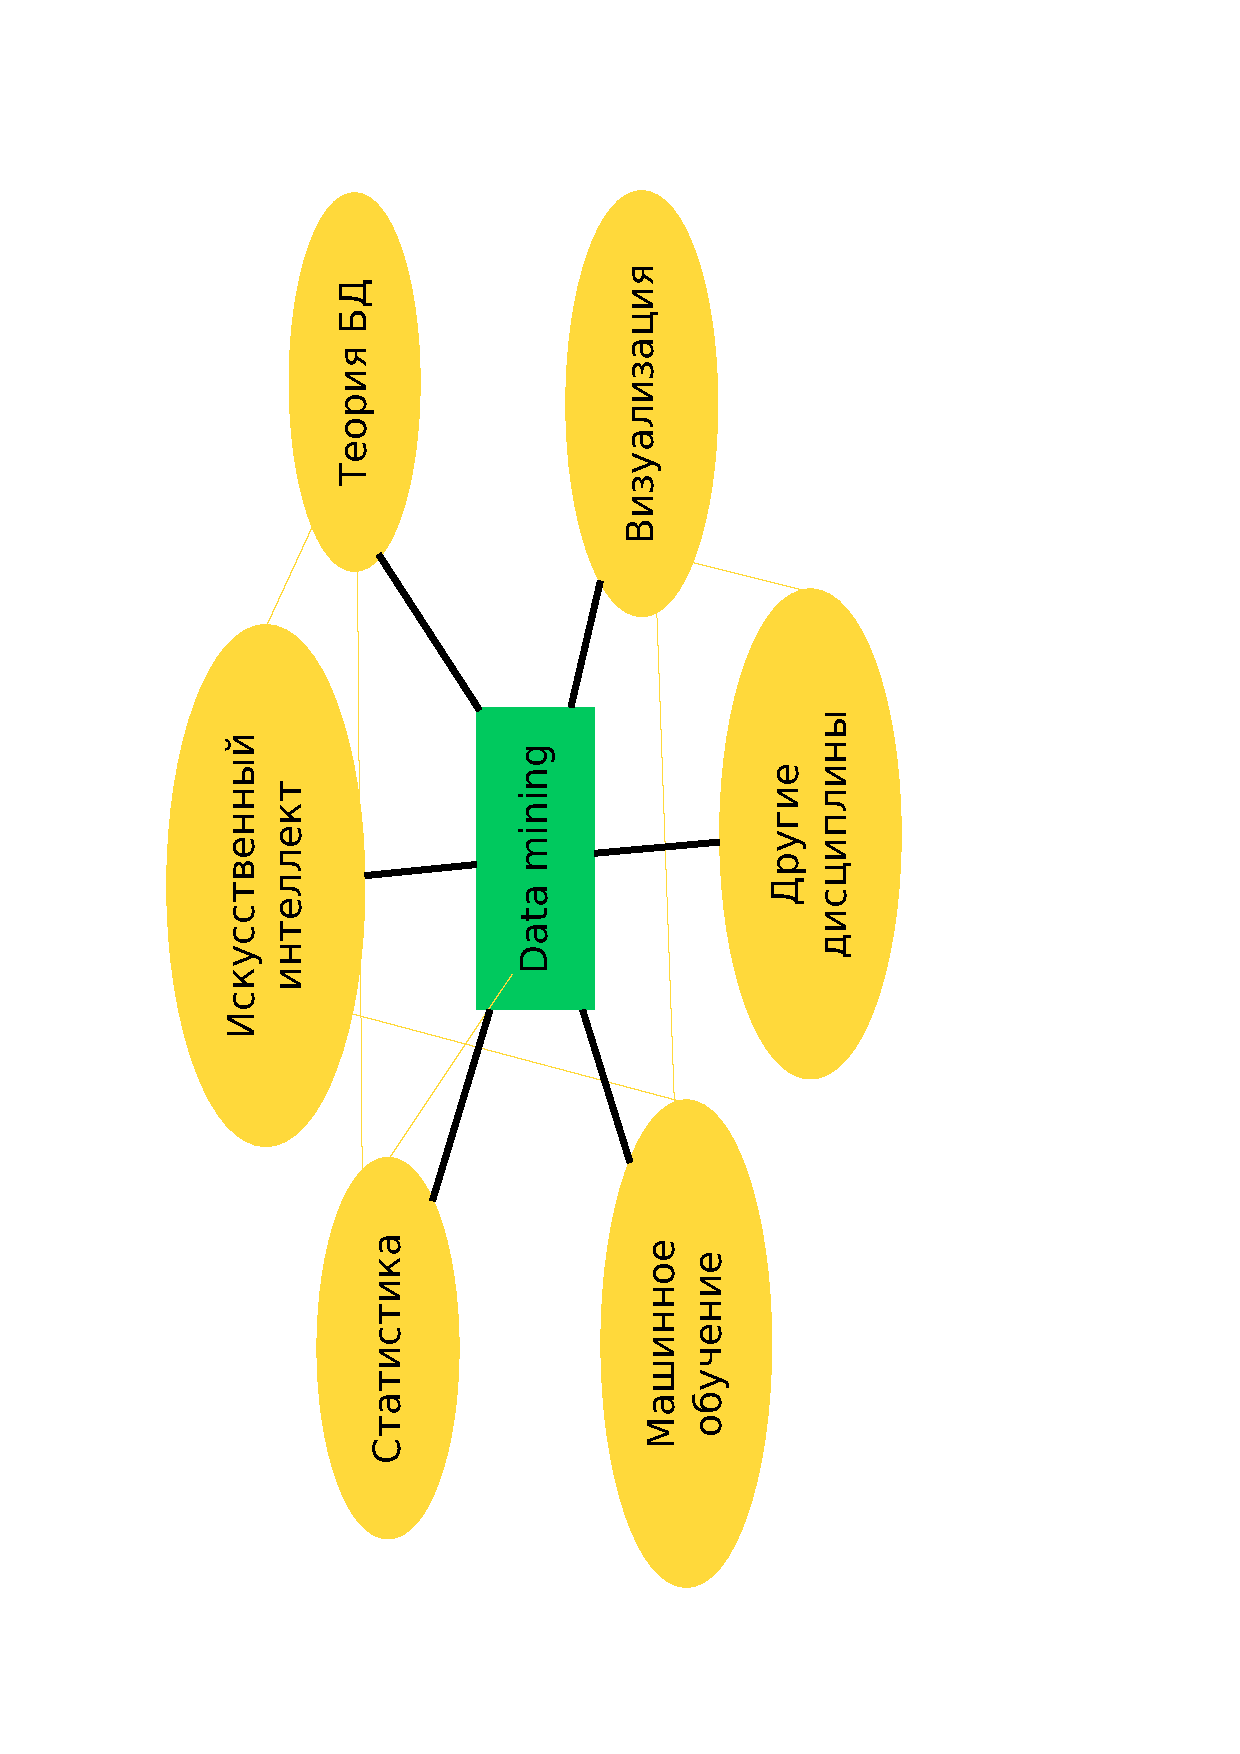
\includegraphics[angle=270,scale=0.3,clip=true,trim=23mm 25mm 53mm 30mm]{data/diag1}}
    \vspace{-5pt}
    \caption{ИАД как мультидисциплинарная наука}
  \end{figure}
\end{frame}

\begin{frame}
  \frametitle{Введение}
  \framesubtitle{Отличия от других методов анализа данных}
  В основу современной технологии Data Mining положена концепция шаблонов (паттернов), отражающих фрагменты многоаспектных взаимоотношений в данных.

  \vspace{-15pt}

  \begin{table}
    \caption{Примеры формулировок задач}
    \vspace{-10pt}
    \begin{tabular}{|p{0.5\textwidth}|p{0.45\textwidth}|}
      \hline
      \cellcolor{cell1} OLAP (online analytical processing) & \cellcolor{cell2} Data Mining \\ \hline
      \cellcolor{cell1} Каковы средние показатели травматизма для курящих и некурящих? & \cellcolor{cell2} Встречаются ли точные
      шаблоны в описаниях людей, подверженных повышенному травматизму? \\ \hline
      \cellcolor{cell1} Каковы средние размеры телефонных счетов существующих клиентов в сравнении со счетами бывших клиентов (отказавшихся от услуг телефонной компании)? &
      \cellcolor{cell2} Имеются ли характерные портреты клиентов, которые, по всей вероятности, собираются отказаться от услуг телефонной компании? \\
      \hline
    \end{tabular}
  \end{table}
\end{frame}

\subsection{Процесс Data Mining}

\begin{frame}
  \frametitle{Процесс Data Mining}
  \framesubtitle{Этапы}

  \begin{enumerate}
    \item Анализ предметной области
    \item Постановка задачи
      \begin{enumerate}
        \item Формулировка
        \item Формализация
      \end{enumerate}
    \item Подготовка данных
    \item Построение моделей
    \item Проверка и оценка моделей
    \item Выбор модели и применение модели
    \item Коррекция и обновление модели
    \end{enumerate}
\end{frame}

\begin{frame}
  \frametitle{Процесс Data Mining}
  \framesubtitle{Данные}
  
  \begin{defn}
    Данные - это необработанный материал, предоставляемый поставщиками \emph{данных} и используемый потребителями для формирования информации.
  \end{defn}

  Наиболее часто встречающиеся (обрабатываемые) данные \footnotemark:
  \begin{enumerate}
    \item Табличные данные
    \item Временные ряды
    \item Текст
    \item Графические данные: изображения, графы, карты, молекулы, web-данные
    \item Аудио/Видео
  \end{enumerate}

  \footnotetext[1]{По данным сайта \url{http://www.kdnuggets.com/}} 
\end{frame}

\begin{frame}
  \frametitle{Процесс Data Mining}
  \framesubtitle{Данные (2)}
  
  \begin{itemize}
  \item Для выполнения основной цели (нахождения шаблонов) нужны большие объемы информации.
    
  \item Для обработки сырых данных потребуется большое количество времени.
  \end{itemize}
  
  \begin{defn}
    Подготовка, предобработка данных - выделение особых, уникальных для предметной области признаков из каждого наблюдения из сырых данных для уменьшения объема обрабатываемой информации и улучшения полученных результатов.
  \end{defn}

\end{frame}


\section{Задачи и методы решения}
%\contentsline {section}{Задачи и методы решения \\}
%\addtocontents{toc}{ \newline}

% \subsection{Основы анализа данных}
% \begin{frame}
%   \frametitle{Основы анализа данных}
%   \framesubtitle{Статистики}
%   \vspace{-30pt}
%   \begin{columns}[t]

%     \begin{column}{0.35\textwidth}
%       \begin{table}
%         \caption{Набор данных A}
%         \begin{tabular}{|c|c|}
%           \hline
%           x & y \\ \hline
%           3 & 9 \\ \hline 2 & 7 \\ \hline 4 & 12 \\ \hline 5 & 15 \\ \hline 6 & 17 \\ \hline
%           7 & 19 \\ \hline 8 & 21 \\ \hline 9 & 23.4 \\ \hline 10 & 25.6 \\ \hline 11 & 27.8 \\
%           \hline
%         \end{tabular}
%       \end{table}
%     \end{column}

%     \begin{column}{0.7\textwidth}
%       \begin{table}
%         \caption{Описательные статистики для набора A}
%         \begin{tabular}{|c|c|c|}
%           \hline
%           Описательная статистика & x & y \\ \hline
%           Среднее & 6,5 & 17,68 \\ \hline
%           Медиана & 6,5 & 18 \\ \hline
%           Стандартное отклонение & 3,02 & 6,99 \\ \hline
%           Дисперсия выборки & 9,16 & 48,88 \\ \hline
%           Эксцесс & -1,2 & -1,10 \\ \hline
%           Асимметричность & 0 & -0,12 \\ \hline
%           Интервал & 9 & 20,8 \\ \hline
%           Минимум & 2 & 7 \\ \hline
%           Максимум & 11 & 27,8 \\ \hline
%           Сумма & 65 & 176,8 \\ \hline
%           Уровень надежности (95,0\%) & 2,16 & 5,00 \\
%           \hline
%         \end{tabular}
%       \end{table}
%     \end{column}
%   \end{columns}
% \end{frame}

\subsection{Регрессия}

\begin{frame}
  \frametitle{Регрессия. Прогнозирование}
  \framesubtitle{Постановка задачи}

  \begin{defn}
    Регрессия — зависимость математического ожидания (например, среднего значения) случайной величины от одной или нескольких других случайных величин (свободных переменных), то есть $E(y|x) = f(x)$.
  \end{defn}
  Применяется для \textbf{прогнозирования} и \textbf{предсказывания}.\\
  Регрессия может быть представлена в виде суммы неслучайной и случайной составляющих.
  \[y = f(x) + \nu\]
  где $f$ — функция регрессионной зависимости, а $\nu$ — аддитивная случайная величина с нулевым матожиданием.
\end{frame}

\begin{frame}
  \frametitle{Регрессия. Прогнозирование}
  \framesubtitle{Постановка задачи (2)}

  \begin{prob}
    Задана выборка — множество $\{x_1, \dots, x_N | x \in R^M\}$ значений свободных переменных и множество $\{y_1, \dots, y_N | y \in R \}$ соответствующих 
    значений зависимой переменной. Задана регрессионная модель -- параметрическое семейство функций $f(w,x)$ зависящих
    от параметров $w \in R^W$ и свободных переменных $x$. Требуется найти наиболее вероятные параметры $\overline{w}$:
    \vspace{-10pt}
    \[
    \overline{w} = \operatorname*{arg\,max}_{w \in R^W}p(y | x, w, f)
    \]
  \end{prob}
\end{frame}

\begin{frame}
  \frametitle{Регрессия. Прогнозирование}
  \framesubtitle{Линейная регрессия}

  Функция $f$ зависит от параметров  линейно:
  \[ y = f(w, x) + \nu = \sum_{j=1}^N{w_j \cdot g_j(x)} + \nu\]
  Значения параметров находят \textbf{методом наименьших квадратов}. \\
  \begin{defn}
  Разности $y_i - f(x_i)$ между фактическими значениями зависимой переменной и восстановленными называются \textbf{регрессионными остатками (residuals)}.
  \end{defn}
  \vspace{-10pt}
  \[SSE~(\text{Sum of Squared Errors}) = |f(x) - y|_2 = \sum_{j=1}^N(y_i - f(x_i))^2\]
  \[MSE~(\text{Mean Square Error}) = \frac{SSE}{N - 2}\]
\end{frame}

\begin{frame}
  \frametitle{Регрессия. Прогнозирование}
  \framesubtitle{Пример}

  \begin{columns}
    \begin{column}{0.5\textwidth}
      \begin{center}
        {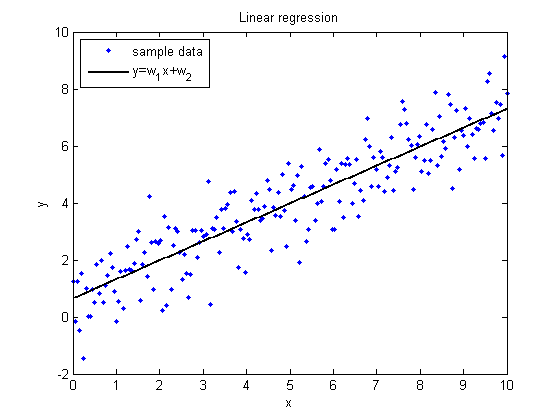
\includegraphics[scale=0.33,clip=true,trim=13mm 3mm 16mm 4mm]{data/regr1.png}}
      \end{center}
    \end{column}
    
    \begin{column}{0.5\textwidth}
      \begin{center}
        {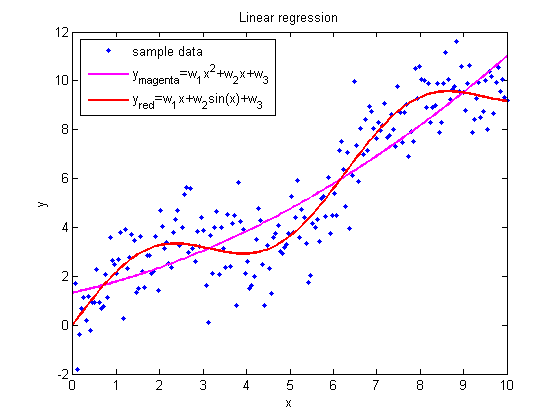
\includegraphics[scale=0.33,clip=true,trim=13mm 3mm 16mm 4mm]{data/regr2.png}}
      \end{center}
    \end{column}
    
  \end{columns}
\end{frame}

\subsection{Машинное обучение}
\begin{frame}
  \frametitle{Машинное обучение}
  \begin{defn}
    Машинное обучение (англ. Machine Learning) — обширный подраздел искусственного интеллекта, изучающий методы построения алгоритмов, способных обучаться.
  \end{defn}

  \vspace{25pt}

  Задачи машинного обучения разделяются на:
  \begin{itemize}
  \item Обучение с учителем    \\
  \item Обучение без учителя
  \end{itemize}
\end{frame}

% \begin{frame}
%   \frametitle{Машинное обучение}
%   \framesubtitle{Обучение с учителем}
% \end{frame}

% \begin{frame}
%   \frametitle{Машинное обучение}
%   \framesubtitle{Обучение без учителя}
% \end{frame}

\subsection{Классификация}
\begin{frame}
  \frametitle{Классификация}
  \framesubtitle{Постановка задачи}
  
  \begin{prob}
    Путь $X$ - множество объектов, $Y$ - конечное множество меток.
    Для элементов данной конечной выборки из $X$ известны метки объектов. Требуется построить алгоритм,
    способный классифицировать произвольный объект $x \in X$.
  \end{prob}

  \vspace{-15pt}

  \begin{center}
    \begin{figure}
      \caption{Пример. Классификация зеленого треугольника}
      \vspace{-5pt}
      \fbox{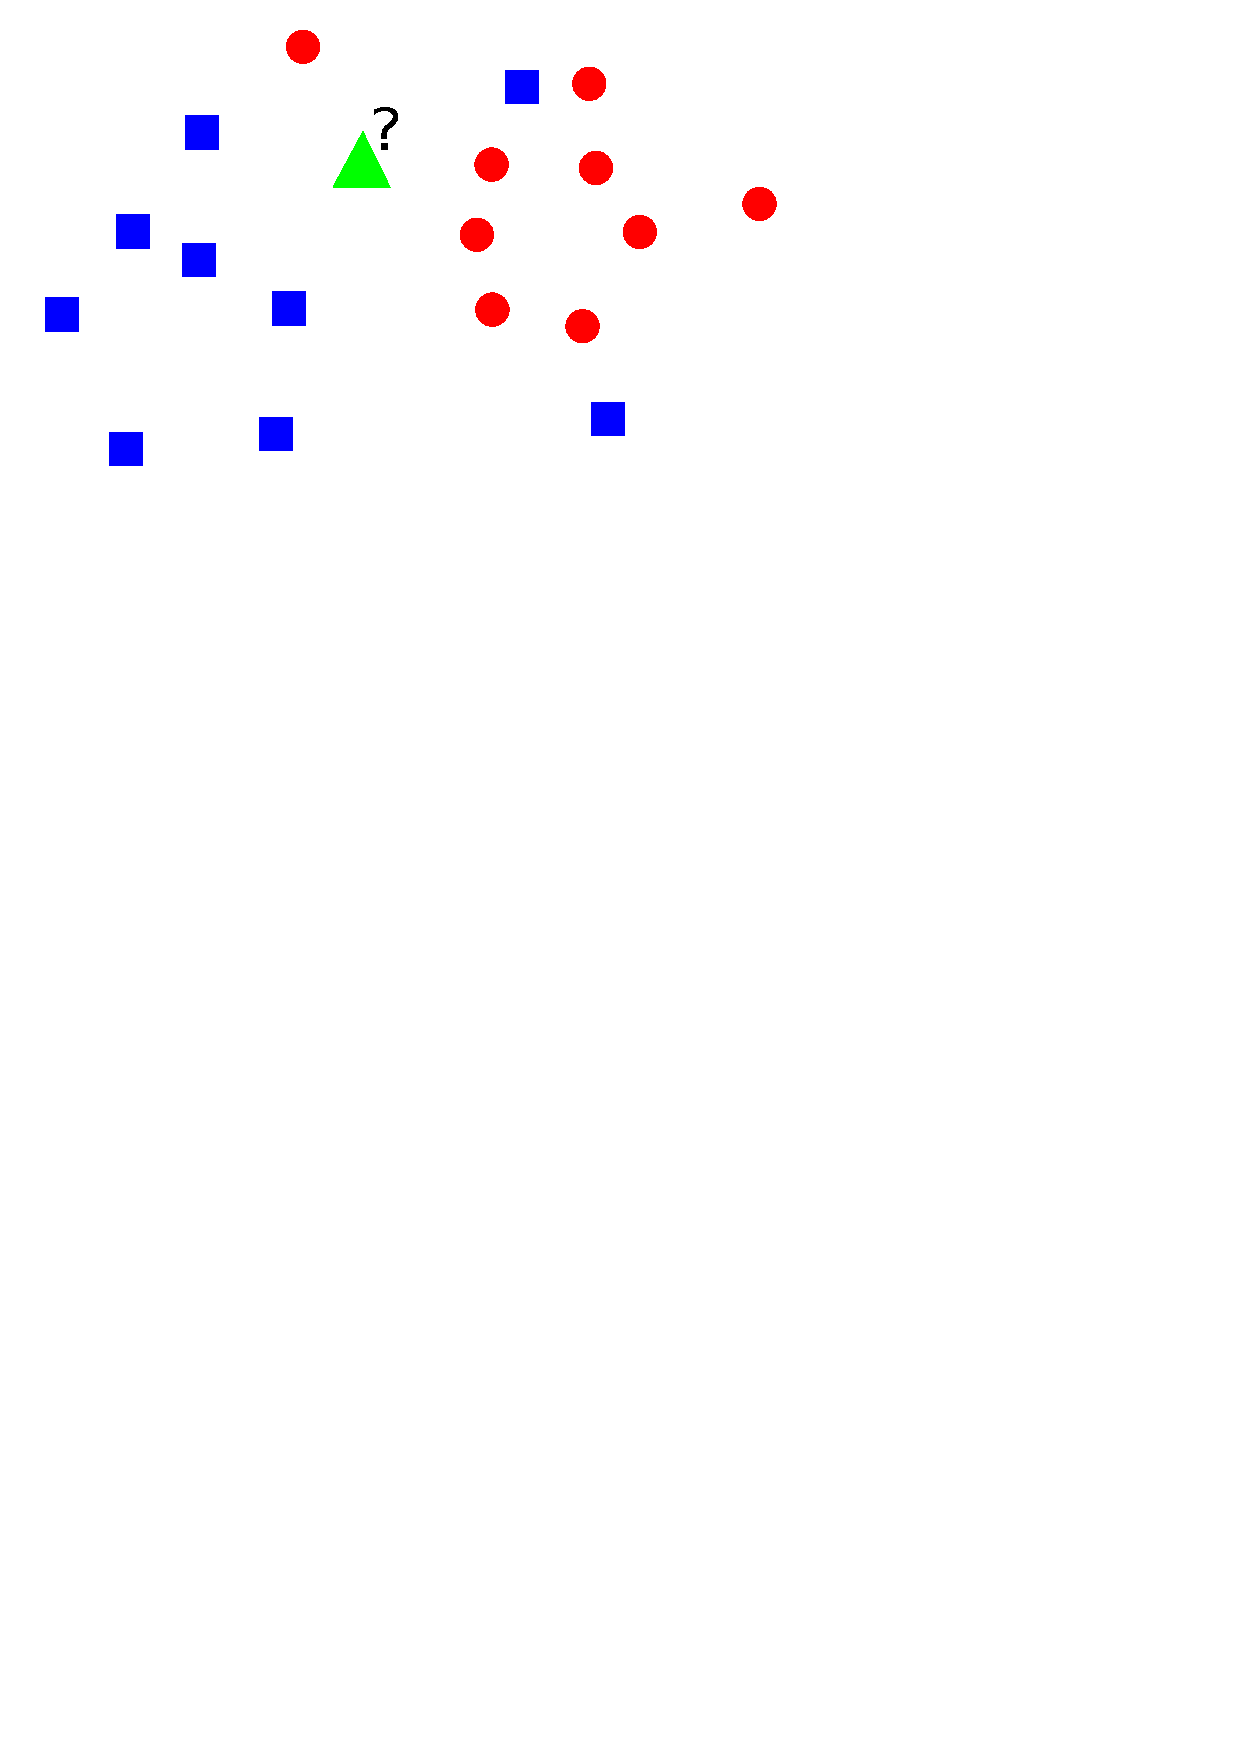
\includegraphics[scale=0.4,clip=true,trim=5mm 215mm 75mm 5mm]{data/class}}
    \end{figure}
  \end{center}
\end{frame}

\begin{frame}
  \frametitle{Классификация}
  \framesubtitle{k ближайших соседей (k-NN)}

  \begin{columns}
    \begin{column}{0.4\textwidth}
      \fbox{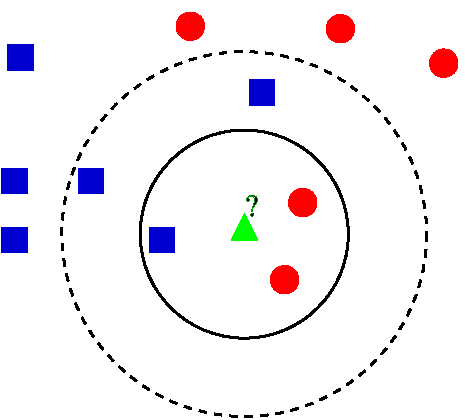
\includegraphics[scale=0.55]{data/knn}}
    \end{column}
    \begin{column}{0.6\textwidth}
      Для произвольного объекта $x$ отсортируем объекты обучающей выборки:
      \[\rho(x, x_{1;x}) < \dots < \rho(x, x_{m;x})\]

      Обобщеная формула классификации:
      \vspace{-10pt}
      \[A(x) = \operatorname*{arg\,max}_{y \in Y}{\sum_{i=1}^m[x_{i;x} = y] \cdot w(i, x)}\]
    \end{column}
  \end{columns}  

  $w(i, x)$ - весовая функция:
  \begin{itemize}
  \item $w(i, x) = [i = 1]$ - метод ближайшего соседа
  \item $w(i, x) = [i \leq k]$ - метод k ближайших соседей
  \item $w(i, x) = [i \leq k] \cdot q^i,~(q < 1)$ - метод k экспоненциально взвешенных ближайших соседей
  \end{itemize}
\end{frame}

\begin{frame}
  \frametitle{Классификация}
  \framesubtitle{Практическое применение}

  \begin{columns}

  \begin{column}{0.5\textwidth}
    {\includegraphics[scale=0.35]{data/faces.png}}
  \end{column}

  \begin{column}{0.5\textwidth}
    \begin{itemize}
    \item Компьютерное зрение:
      \begin{itemize}
      \item OCR
      \item Системы слежения
      \end{itemize}
    \item Создание новых лекарств. QSAR
    \item Распознавание речи
    \item Поисковые системы
    \item Обработка естественных языков
    \end{itemize}
    \end{column}
  \end{columns}
\end{frame}


\subsection{Клаcтеризация}
\begin{frame}
  \frametitle{Кластеризация}
  \framesubtitle{Постановка задачи}

  \begin{center}
    \fbox{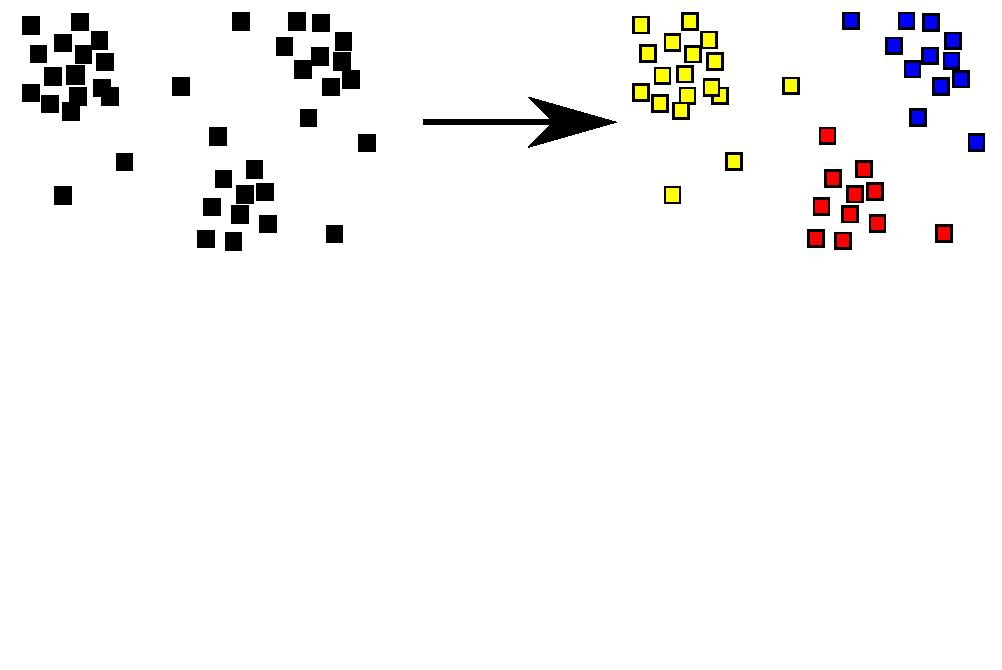
\includegraphics[scale=0.5,clip=true,trim=0mm 70mm 0mm 0mm]{data/cluster}}
  \end{center}

  \vspace{15pt}

  \begin{prob}
    Требуется разбить заданную выборку на непересекающиеся подмножества, называемые \emph{кластерами}, так, чтобы каждый кластер состоял из объектов, близких по метрике,
    а объекты разных кластеров существенно отличались.
  \end{prob}
\end{frame}

\begin{frame}
  \frametitle{Кластеризация}
  \framesubtitle{Типы кластеризации}

  \begin{columns}
    \begin{column}{0.4\textwidth}
      Методы кластерного анализа можно разделить на две группы:
      \begin{itemize}
      \item иерархические
      \item неиерархические
      \end{itemize}
    \end{column}
    
    \begin{column}{0.6\textwidth}
      Иерархические:
      \fbox{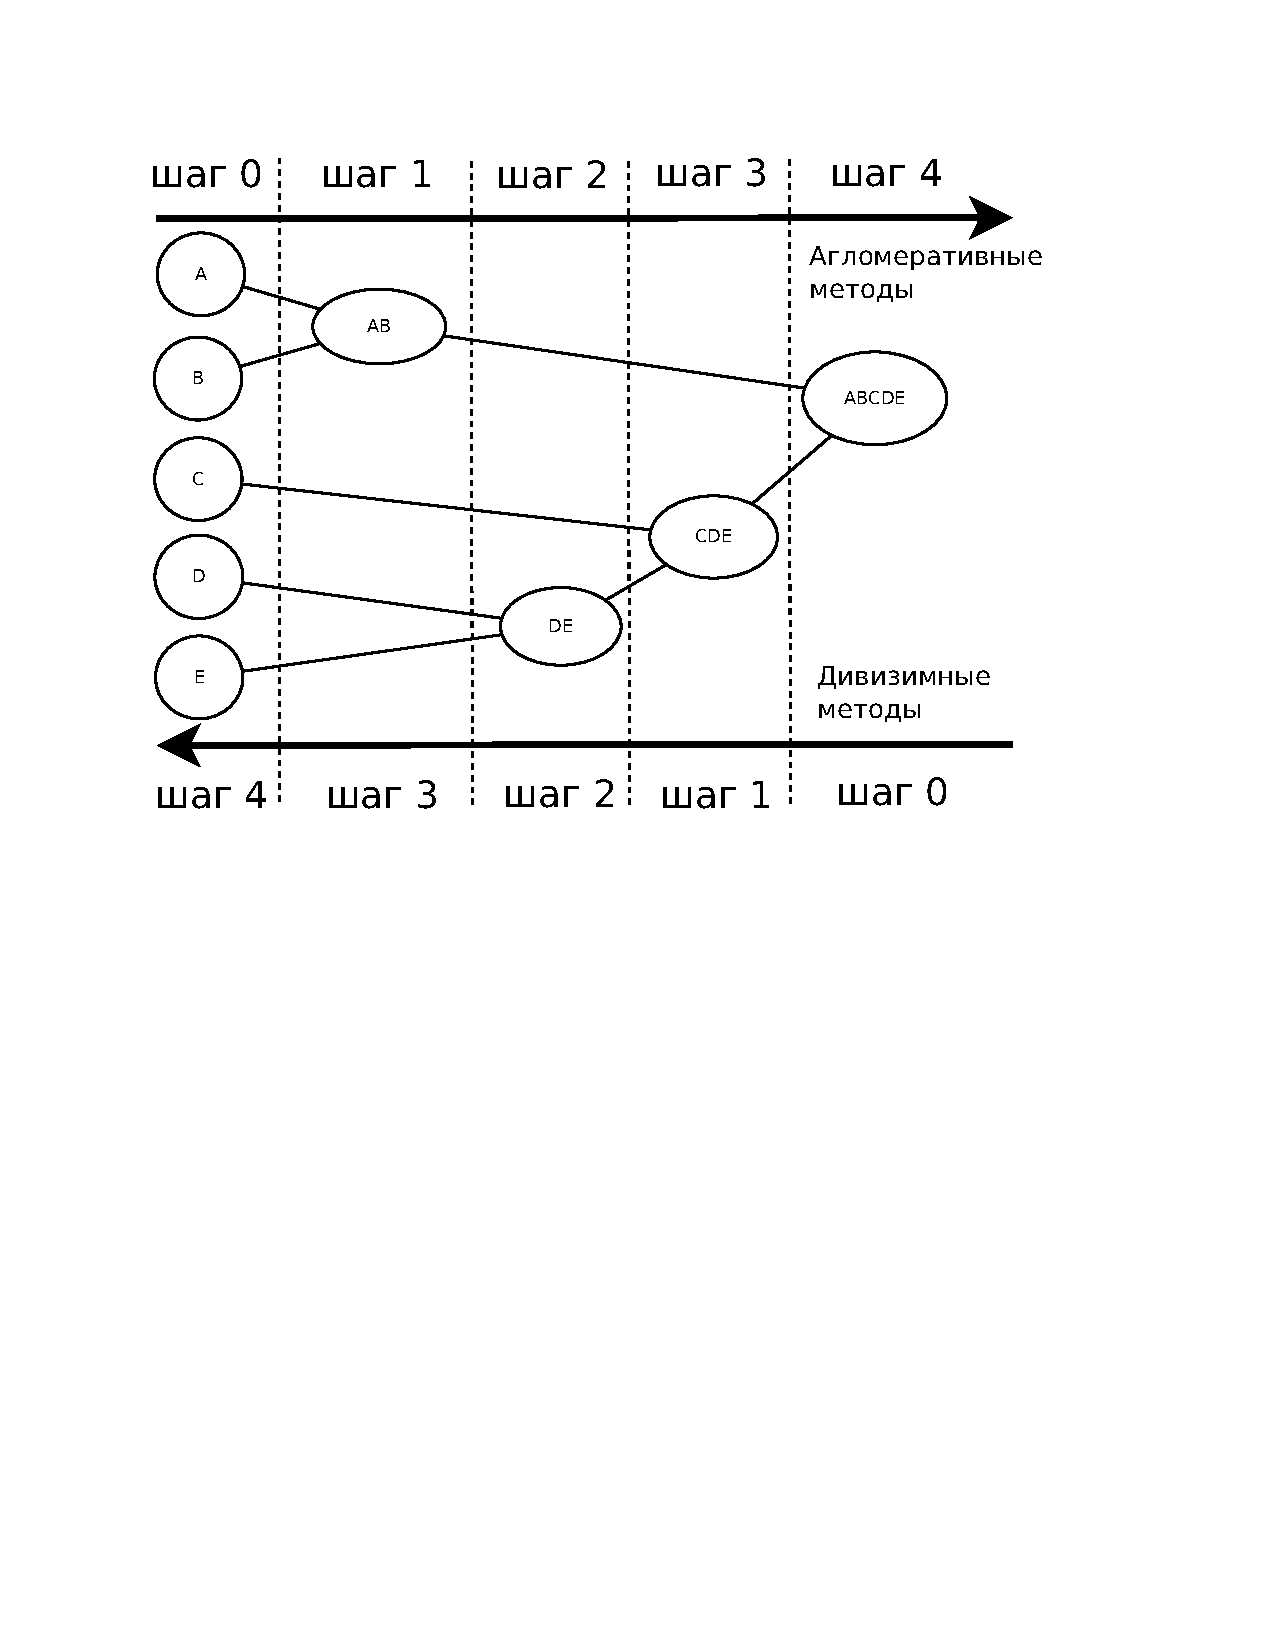
\includegraphics[scale=0.4,clip=true,trim=25mm 140mm 37mm 25mm]{data/hierarchical}}
    \end{column}
   
  \end{columns}
  \begin{defn}
    Дендрограмма (dendrogram) - древовидная диаграмма, содержащая n уровней, каждый из которых соответствует одному из шагов процесса последовательного укрупнения кластеров.
  \end{defn}
  
\end{frame}

\begin{frame}
  \frametitle{Кластеризация}
  \framesubtitle{Иерархическая кластеризация}

  \begin{center}
    Основная идея - объединение близко расположенных кластеров
  \end{center}

  \begin{columns}
    \begin{column}{0.5\textwidth}
      Исходные данные:
      \fbox{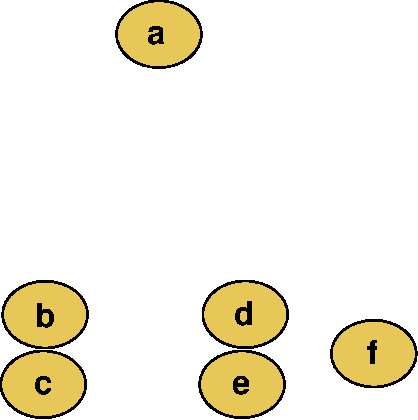
\includegraphics[scale=0.5]{data/clusters_orig}}

      Типичные функции расстояния между кластерами $A, B$:
      \begin{itemize}
      \item $\max\{d(x, y): x \in A, y \in B\}$
      \item $\min\{d(x, y): x \in A, y \in B\}$
      \item $\frac{1}{|A| \cdot |B|} \sum_{x \in A}\sum_{y \in B}d(x, y)$
      \end{itemize}
    \end{column}

    \begin{column}{0.5\textwidth}
      Дендрограмма кластеризации:
      \fbox{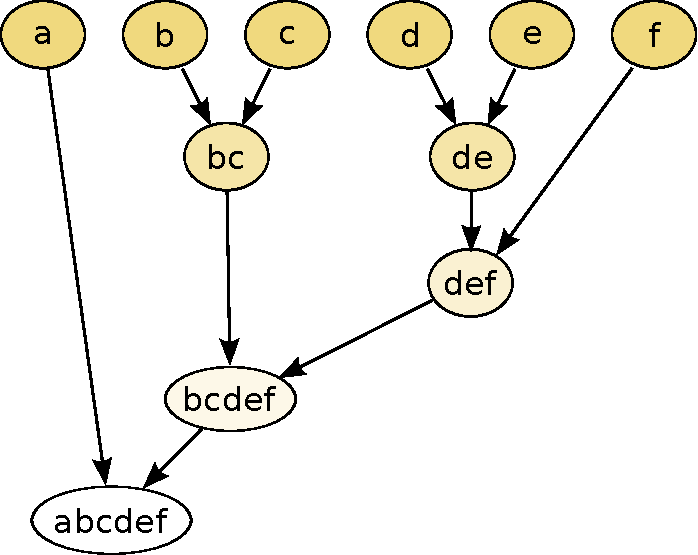
\includegraphics[scale=0.48]{data/clusters_dendr}}
    \end{column}
  \end{columns}
\end{frame}

\begin{frame}
  \frametitle{Кластеризация}
  \framesubtitle{k средних}

  \begin{columns}
    \begin{column}{0.5\textwidth}
      \begin{center}
        \fbox{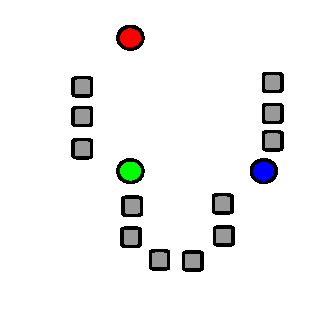
\includegraphics[scale=0.5,clip=true,trim=0mm 7.5mm 0mm 0mm]{data/km-s1}}
        \\Шаг 1. Выбор начальных центров кластеров.       
        
        \fbox{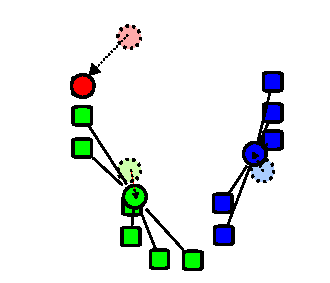
\includegraphics[scale=0.5,clip=true,trim=0mm 1.5mm 0mm 0mm]{data/km-s3}}
        \\Шаг 3. Вычисление новых центров.
      \end{center}
    \end{column}
    
    \begin{column}{0.5\textwidth}
      \begin{center}
        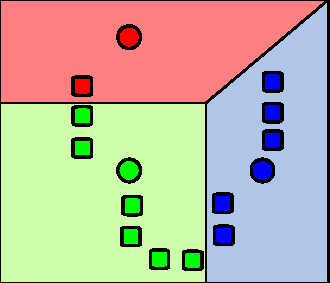
\includegraphics[scale=0.5]{data/km-s2}
        \\Шаг 2. Создание k кластеров. Диаграмма Вороного.

        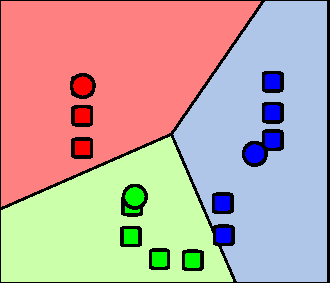
\includegraphics[scale=0.5]{data/km-s4}
        \\Шаг 4. Повторять шаги 2, 3, пока кластеры изменяются.
      \end{center}
    \end{column}
  \end{columns}
\end{frame}

\begin{frame}
  \frametitle{Кластеризация}
  \framesubtitle{Практическое применение}

  \begin{columns}
    \begin{column}{0.4\textwidth}
      \begin{figure}
        \includegraphics[scale=0.08]{data/cluster_gene}
        \caption{Кластеризация генов}
        \end{figure}
    \end{column}
    
    \begin{column}{0.6\textwidth}
      \begin{itemize}
      \item Группирование результатов поиска
      \item Сегментация изображения
      \item Может быть использован для дифференцирования различных тканей и крови на ПЭТ-снимках
      \item Нахождение сообществ в социальных сетях
      \item Разделение web-страниц по жанрам
      \end{itemize}
    \end{column}
  \end{columns}
\end{frame}

\subsection{Задача сокращения размерности}
\begin{frame}
  \frametitle{Задача сокращения размерности}
  \framesubtitle{Постановка задачи}

  \begin{prob}
    Исходная информация - признаковые описания (число признаков может быть большим).
    Необходимо представить эти данные в пространстве меньшей размерности, по возможности, минимизировав потери информации.
  \end{prob}
  \vspace{15pt}
  \textbf{Метод главных компонент} -- К. Пирсон, 1901г
  \vspace{5pt}
  \begin{prob}
    Аппроксимировать данные линейными многообразиями меньшей размерности.
  \end{prob}
\end{frame}

\begin{frame}
  \frametitle{Задача сокращения размерности}
  \framesubtitle{Метод главных компонент}

  \begin{enumerate}
    \item Организация данных
      \[ X = [x_1, x_2, ..., x_N]~\text{-- исходный набор данных размерности}~N\]
      \[x_i = \begin{pmatrix} x_{i,1} \\ \vdots \\ x_{i, M} \end{pmatrix} \]
    \item Централизация
      \[ u[m] = \frac{1}{N}\sum_{n=1}^{N}X[m,n], m = 1, \dots M ~\text{-- вектор-столбец средних} \]
      \[ B = X - u \cdot \underbrace{\begin{pmatrix} 1, \dots, 1 \end{pmatrix}}_\text{N} \]
    \item Матрица ковариаций
      \[ C = \mathbb{E}[B \cdot B^*] = \frac{1}{N} \sum B \cdot B^*\]
  \end{enumerate}
\end{frame}

\begin{frame}
  \frametitle{Задача сокращения размерности}
  \framesubtitle{Метод главных компонент (2)}

  \begin{enumerate}
    \setcounter{enumi}{3}
    \item Собственные числа (СЧ) и вектора (СВ) \\
      Найти матрицы $V$ -- матрица СВ и $D$ -- диагональная матрица СЧ:
      \[V^{-1}CV = D\]
    \item Отсортировать СВ и СЧ в порядке убывания последних
    \item Сосчитать суммарную энергию данных для каждого СВ
      \vspace{-5pt}
      \[g[m] = \sum_{q=1}^m D[q, q], m = 1,\dots,M \]
      \vspace{-5pt}
    \item Выбор нового базиса
      \[W[p, q] = V[p, q], \begin{array} {l} p = 1, \dots, M \\ q = 1, \dots, L \end{array} \]
      \begin{center}$L$ - новая размерность, $L < M$ \end{center}
    \item Трансформирование данных
      \[Y = W^* \cdot X \]
  \end{enumerate}
\end{frame}

\begin{frame}
  \frametitle{Задача сокращения размерности}
  \framesubtitle{Применения}

  \begin{columns}
    \begin{column}{0.44\textwidth}
      \begin{itemize}
      \item \textbf{Визуализация данных}
        \vspace{1pt}
      \item Компрессия изображений
        \vspace{5pt}
      \item Подавление шума на изображениях
        \vspace{5pt}
      \item Хемометрика
        \vspace{5pt}
      \item Биоинформатика
      \end{itemize}
    \end{column}
  
    \begin{column}{0.56\textwidth}
      {\includegraphics[scale=0.3,clip=true,trim=30mm 22mm 50mm 90mm]{data/pca.png}}
    \end{column}

  \end{columns}
\end{frame}


\subsection{Поиск ассоциативных правил}
\begin{frame}
  \frametitle{Поиск ассоциативных правил}
  \framesubtitle{Постановка задачи}

  \begin{center}
    Пример задачи \\ \vspace{10pt}
    \begin{tabular}{|c|c|}
      \hline
      Транзакция & Покупки \\ \hline
      1 & хлеб, молоко, печенье \\ \hline
      2 & молоко, сметана \\ \hline
      3 & молоко, хлеб, сметана, печенье \\ \hline
      4 & колбаса, сметана \\ \hline
      5 & хлеб, молоко, печенье, сметана \\ \hline
      6 & конфеты \\ \hline
    \end{tabular}
    \[ \Downarrow \]
    \[ \{\text{хлеб}, \text{печенье}\} \Rightarrow \{\text{молоко}\}; \{\text{сметана}\} \Rightarrow \{\text{молоко}\} \]
  \end{center}  

  \begin{defn}
    Правило вида <<Из события A следует B>> называется ассоциативным.
  \end{defn}
\end{frame}

\begin{frame}
  \frametitle{Поиск ассоциативных правил}
  \framesubtitle{Характеристики правил}

  \begin{defn}
    \textbf{Поддержкой (supp)} правила называется кол-во или процент транзакций, содержащий набор данных правила.
  \end{defn}

  \[ \text{supp}(\{\text{хлеб}, \text{печенье}, \text{молоко}\}) = 3 \]

  \begin{defn}
    \textbf{Достоверность} правила -- вероятность того, что из события A следует B.
  \end{defn}

  \begin{center}
    Достоверность правила <<из покупки молока следует покупка печенья>> равна 75\%
  \end{center}
\end{frame}

\begin{frame}
  \frametitle{Поиск ассоциативных правил}
  \framesubtitle{Метод <<Априори>>}
  
  \begin{enumerate}
    \item Задается минимальный уровень поддержки (в примере -- 3)
    \item \textbf{Формирование} и \textbf{подсчет} 1-элементных наборов, 2-элементных, 3-элементных... \\
  \end{enumerate}

  \begin{columns}[t]
   
    \begin{column}{0.3\textwidth}
      \begin{center}
        Шаг 2.1
        \begin{tabular}{|c|c|}
          \hline
          Набор & supp \\ \hline
          \cellcolor{cell2} Х & \cellcolor{cell2} 3 \\ \hline
          \cellcolor{cell2} М & \cellcolor{cell2} 4 \\ \hline
          \cellcolor{cell2} П & \cellcolor{cell2} 4 \\ \hline
          \cellcolor{cell2} С & \cellcolor{cell2} 3 \\ \hline
          Кл & 1 \\ \hline
          Кф & 1 \\ \hline
        \end{tabular}
      \end{center}
    \end{column}

    \begin{column}{0.3\textwidth}
      \begin{center}
        Шаг 2.2
        \begin{tabular}{|c|c|}
          \hline
          Набор & supp \\ \hline
          \cellcolor{cell2} ХМ & \cellcolor{cell2} 3 \\ \hline
          \cellcolor{cell2} ХП & \cellcolor{cell2} 3 \\ \hline
          ХС & 2 \\ \hline
          МП & 2 \\ \hline
          \cellcolor{cell2} МС & \cellcolor{cell2} 3 \\ \hline
          ПС & 2 \\ \hline
        \end{tabular}
      \end{center}
    \end{column}

    \begin{column}{0.3\textwidth}
      \begin{center}
        Шаг 2.3
        \begin{tabular}{|c|c|}
          \hline
          Набор & supp \\ \hline
          \cellcolor{cell2} ХМП & \cellcolor{cell2} 3 \\ \hline
          ХМС & 2 \\ \hline
          МПС & 2 \\ \hline
          ХПС & 2 \\ \hline
        \end{tabular}
      \end{center}
    \end{column}
    
  \end{columns}

\end{frame}

\section{Программные продукты}
\subsection{Deep Data Diver}
\begin{frame}
  \frametitle{Программные продукты}
  \framesubtitle{Deep Data Diver}
  \begin{center}
    \vspace{-5pt}
    Система поиска ассоциативных правил. Разработка РАН. \\
    \vspace{5pt}
    
    {\includegraphics[scale=0.51]{data/ddd.png}}
    
    \vspace{5pt}
  
    Использует аппарат линейной алгебры и процедуры самоорганизации данных.
  \end{center}  
\end{frame}

\subsection{Poly Analyst}
\begin{frame}
  \frametitle{Программные продукты}
  \framesubtitle{Poly Analyst}
  \begin{columns}[t]
    \begin{column}{0.5\textwidth}
      Решаемые задачи:
      \begin{center}
        \begin{itemize}
          \item Классификация
          \item Кластеризация
          \item Предсказывание, анализ трендов
          \item Поиск ассоциативных правил
          \item Визуализация
          \item Обработка естественных языков
          \item ...
        \end{itemize}
      \end{center}
    \end{column}
    
    \begin{column}{0.5\textwidth}
      Доступные методы:
      \begin{center}
        \begin{itemize}
          \item Различные классификаторы
          \item Машины опорных векторов
          \item Нейронные сети
          \item Корреляционный, регрессионный анализ
          \item ...
        \end{itemize}
      \end{center}

      \includegraphics[scale=0.19]{data/pa}
    \end{column}
    
  \end{columns}
\end{frame}

\subsection{Oracle Data Mining}
\begin{frame}
  \frametitle{Программные продукты}
  \framesubtitle{Oracle Data Mining}
  \vspace{-25pt}
  \begin{center}
    {\includegraphics[scale=0.4]{data/odmlogo.png}}
  \end{center}

  
  \begin{columns}[t]
     \begin{column}{0.5\textwidth}
       Решаемые задачи:
       \vspace{-5pt}
       \begin{center}
         \begin{itemize}
           \item Классификация
           \item Кластеризация
           \item Предсказывание
           \item Поиск ассоциативных правил
           \item Визуализация
           \item Нахождение аномалий
         \end{itemize}
       \end{center}
     \end{column}
    
     \begin{column}{0.5\textwidth}
       Доступные методы:
       \vspace{-5pt}
       \begin{center}
         \begin{itemize}
           \item Различные классификаторы
           \item Машины опорных векторов
           \item {<<Априори>>}
           \item Регрессионный анализ
           \item Деревья решений
           \item ...
         \end{itemize}
       \end{center}
     \end{column}
   \end{columns}
\end{frame}

\begin{frame}
  \frametitle{Программные продукты}
  \framesubtitle{Oracle Data Mining (2)}
  \begin{center}
    \includegraphics[scale=0.23]{data/odm.png}
  \end{center}
\end{frame}


\section*{Заключение}
\begin{frame}
  \frametitle{Заключение}

  \begin{itemize}
    \item Рынок систем Data Mining экспоненциально развивается
    \item Системы Data Mining применяются по двум основным направлениям:
      \begin{itemize}
        \item как массовый продукт для бизнес-приложений
        \item как инструменты для проведения уникальных исследований (генетика, химия, медицина и пр.)
      \end{itemize}
    \item Data mining - не панацея. Всё зависит от подготовки и качества данных
  \end{itemize}
\end{frame}

\begin{frame}
  \frametitle{Список литературы}

  \begin{enumerate}
    \item Википедия (англ., рус.)
    \item \url{http://www.machinelearning.ru}
    \item \url{http://www.intuit.ru/department/database/datamining}
    \item \url{http://www.inftech.webservis.ru/it/database/datamining/ar2.html}
    \item \url{http://www.oracle.com/technetwork/database/options/odm/index.html}
    \item \url{http://www.megaputer.com/polyanalyst.php}
    \item \url{http://datadiver.nw.ru/prod_dd.htm}
  \end{enumerate}
\end{frame}


\begin{frame}
  \frametitle{}
  \framesubtitle{}

  \begin{center}\LARGE{Спасибо за внимание!}\end{center}
\end{frame}

\end{document}